\documentclass[a4paper,14pt]{extarticle}

\usepackage[T2A]{fontenc}
\usepackage[utf8]{inputenc}
\usepackage[english,russian]{babel}
\usepackage{indentfirst}
\usepackage{setspace}
\usepackage{geometry}
\geometry{a4paper,left=30mm,right=15mm,top=20mm,bottom=20mm}
\onehalfspacing
\setlength{\parindent}{1.25cm}

% Выравнивание заголовков по ГОСТ ИТМО
\usepackage{titlesec}
\titleformat{\section}[block]
{\centering\bfseries\Large}{\thesection}{1em}{}
\titleformat{\subsection}[block]
{\centering\bfseries\large}{\thesubsection}{1em}{}
\titleformat{\subsubsection}[block]
{\centering\bfseries\normalsize}{\thesubsubsection}{1em}{}

% Настройка подписей к рисункам по ГОСТ (номер и текст по центру)
\usepackage{caption}
\captionsetup[figure]{
    justification=centering,
    labelsep=endash,
    font=small,
    name=Рисунок,
    singlelinecheck=true
}

% Нумерация страниц по ГОСТ (снизу по центру)
\usepackage{fancyhdr}
\pagestyle{fancy}
\fancyhf{}
\fancyfoot[C]{\hspace{-15mm}\thepage}
\renewcommand{\headrulewidth}{0pt}

% Формат списков по ГОСТ
\usepackage{enumitem}
\setlist{nosep, leftmargin=1.25cm}
\setlist[itemize]{label=\raisebox{0.3ex}{\tiny$\bullet$}, labelsep=0.5em}

% Ссылки и математика
\usepackage{hyperref}
\hypersetup{
    colorlinks=true,
    linkcolor=black,
    urlcolor=black,
    citecolor=black
}
\usepackage{amsmath}
\usepackage{graphicx}

% Разрешить более свободный перенос длинных строк
\sloppy

% Команды для удобства
\newcommand{\sectionbreak}{\clearpage}
\newcommand{\img}[3]{%
    \begin{figure}[H]
    \centering
    \includegraphics[width=#1\textwidth]{#2}
    \caption{#3}
    \label{fig:#2}
    \end{figure}
}

\begin{document}
    \thispagestyle{empty}
    \begin{center}
    {\Large\textbf{ФЕДЕРАЛЬНОЕ ГОСУДАРСТВЕННОЕ АВТОНОМНОЕ ОБРАЗОВАТЕЛЬНОЕ УЧРЕЖДЕНИЕ ВЫСШЕГО ОБРАЗОВАНИЯ}}
        \\
        {\Large\textbf{«НАЦИОНАЛЬНЫЙ ИССЛЕДОВАТЕЛЬСКИЙ УНИВЕРСИТЕТ ИТМО»}}\\[5mm]
        {\large ФАКУЛЬТЕТ ТЕХНОЛОГИЙ ИСКУССТВЕННОГО ИНТЕЛЛЕКТА}\\[5mm]
        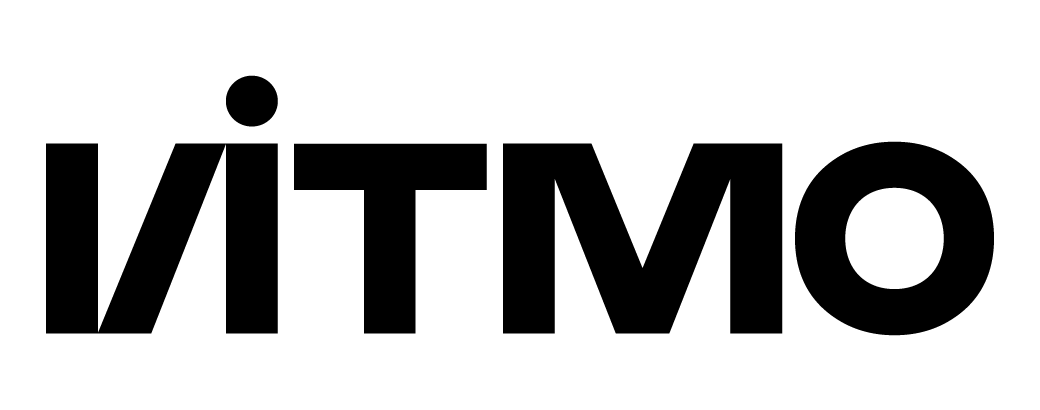
\includegraphics[scale=0.14]{logo.png}\\[20mm]
        \rule{\textwidth}{0.4mm}\\[3mm]
        {\Large Отчёт по лабораторной работе № 5}\\[3mm]
        {\Large по дисциплине «Алгоритмы и структуры данных»}\\[3mm]
        {\Large Hard 7}\\
        \rule{\textwidth}{0.4mm}
    \end{center}
    \vfill
    \begin{flushright}
        \large Выполнил: \\
        Студент группы J3111 \\
        Воробьев Андрей Павлович \\
        ИСУ: 465440 \\
        Преподаватель практики: \\
        Вершинин В.К.
    \end{flushright}
    \vfill
    \begin{center}
        \large Санкт-Петербург \\
        \large 2025
    \end{center}
    \newpage


% =============================================
% Введение
% =============================================
    \section*{1. Введение}
    \subsection*{Цель работы}

    Разработать и оценить алгоритм определения положения абонента на плоскости
    по координатам и расстояниям до ближайших вышек сотовой связи.

    \subsection*{Выполненные задачи}
    \begin{enumerate}
        \item Реализовать функции вычисления расстояний по географическим координатам.
        \item Спроецировать широту/долготу в локальную декартову систему (метры) и обратно.
        \item Сделать два алгоритма:
        \begin{itemize}
            \item «дуогуляцию» (две вышки → две возможные точки).
            \item «мультилатерацию» (больше двух вышек → одна точка).
        \end{itemize}
        \item Объединить всё в единый интерфейс (\textbf{get\_user\_position}).
        \item Оценить качество по всем абонентам: абсолютные и нормированные ошибки; доля попаданий в радиус 50 м.
    \end{enumerate}

% =============================================
% Теоретическая часть
% =============================================
    \section*{2. Теоретическая часть}
    \subsection*{Цилиндрическая проекция}

    \subsubsection*{Формула:}
    \begin{equation}
        \begin{aligned}
            x &= R \cdot (\lambda - \lambda_0) \cdot \cos(\phi_0), \\
            y &= R \cdot \phi,
        \end{aligned}
    \end{equation}

    где:
    \begin{itemize}
        \item $R$ — радиус Земли,
        \item $\phi, \lambda$ — широта и долгота точки (в радианах),
        \item $\phi_0, \lambda_0$ — широта и долгота опорного (центроидного) меридиана.
    \end{itemize}

    \subsubsection*{Вывод и обоснование:}
    \begin{itemize}
        \item Цилиндрическая проекция моделирует Землю как цилиндр, обёрнутый вокруг экватора.
        \item При развертке цилиндра вдоль долготы, меридианы становятся вертикальными прямыми, а параллели — горизонтальными.
        \item долготы $(\lambda - \lambda_0)$ масштабируется поправкой $\cos(\phi_0)$, чтобы учесть сжатие меридианов к полюсам.
        \item Проекция является приближением, точным вдоль параллели $\phi_0$ и достаточно точным для локальных областей (до 20 км).
    \end{itemize}

    \subsection*{Формула гаверсина (Haversine)}

    \subsubsection*{Формула:}
    \begin{equation}
        a = \sin^2\left(\frac{\Delta\phi}{2}\right) + \cos(\phi_1) \cdot \cos(\phi_2) \cdot \sin^2\left(\frac{\Delta\lambda}{2}\right),
    \end{equation}
    \begin{equation}
        d = 2R \cdot \arcsin\left( \sqrt{a} \right),
    \end{equation}

    где:
    \begin{itemize}
        \item $R$ — радиус Земли,
        \item $\phi_1, \phi_2$ — широты двух точек (в радианах),
        \item $\lambda_1, \lambda_2$ — долготы двух точек (в радианах),
        \item $\Delta\phi = \phi_2 - \phi_1$ — разница широт,
        \item $\Delta\lambda = \lambda_2 - \lambda_1$ — разница долгот.
    \end{itemize}

    \subsubsection*{Вывод и обоснование:}

    \begin{itemize}
        \item \textbf{Центральный угол:} между двумя точками на сфере центральный угол \( \theta \) выражается через сферический косинус:
        \[
            \cos \theta = \sin \varphi_1 \sin \varphi_2 + \cos \varphi_1 \cos \varphi_2 \cos(\Delta \lambda).
        \]
        Расстояние по дуге:
        \[
            d = R \cdot \theta.
        \]

        \item \textbf{Переход к гаверсину:} определим гаверсин как:
        \[
            \operatorname{hav}(x) = \sin^2\left(\frac{x}{2}\right) = \frac{1 - \cos x}{2}.
        \]
        Тогда:
        \[
            \operatorname{hav}(\theta) = \frac{1 - \cos \theta}{2}.
        \]

        \item \textbf{Подстановка и преобразование:} подставим выражение из закона косинусов:
        \[
            \operatorname{hav}(\theta) = \frac{1}{2}\left(1 - \left[\sin \varphi_1 \sin \varphi_2 + \cos \varphi_1 \cos \varphi_2 \cos(\Delta \lambda)\right] \right).
        \]
        Воспользуемся тождеством:
        \[
            \cos(\Delta \lambda) = 1 - 2\sin^2\left(\frac{\Delta \lambda}{2}\right),
        \]
        и аналогично:
        \[
            1 - \cos(\theta) = 2 \cdot \operatorname{hav}(\theta).
        \]
        После упрощения получаем:
        \[
            \operatorname{hav}(\theta) = \sin^2\left(\frac{\Delta \varphi}{2}\right) + \cos \varphi_1 \cos \varphi_2 \sin^2\left(\frac{\Delta \lambda}{2}\right).
        \]

        \item \textbf{Расчёт расстояния:} пусть:
        \[
            a = \operatorname{hav}(\theta),
        \]
        тогда:
        \[
            \theta = 2 \arcsin(\sqrt{a}) \quad \Rightarrow \quad d = R \cdot \theta = 2R \cdot \arcsin(\sqrt{a}).
        \]

        \item \textbf{Итоговая формула:}
        \[
            a = \sin^2\left(\frac{\Delta\varphi}{2}\right) + \cos \varphi_1 \cdot \cos \varphi_2 \cdot \sin^2\left(\frac{\Delta\lambda}{2}\right),
        \]
        \[
            d = 2R \cdot \arcsin\left(\sqrt{a}\right).
        \]
    \end{ite  mize}
    \subsubsection*{Преимущества и обоснование:}
    \begin{itemize}
        \item Формула гаверсина устойчива при малых расстояниях и углах.
        \item Избегает численной ошибки, связанной с вычислением $\arccos$ при углах близких к 0.
        \item Часто применяется в навигационных и географических задачах.
    \end{itemize}


    \subsection*{Алгоритм DBSCAN}

    \subsubsection*{Идея:}
    Выделение кластеров по плотности точек без знания числа кластеров заранее.
    Основная информация и идеи реализации взяты из статьи \href{https://proproprogs.ru/ml/ml-algoritm-klasterizacii-dbscan}{Алгоритм кластеризации DBSCAN}.

    \subsubsection*{Параметры:}
    \begin{itemize}
        \item $\varepsilon$ (eps) — радиус окрестности,
        \item $\text{min\_samples}$ — минимальное число точек (включая ядро) в $\varepsilon$-окрестности для образования кластера.
    \end{itemize}

    \subsubsection*{Основные шаги:}
    \begin{itemize}
        \item \textbf{Core point:} точка, у которой в радиусе $\varepsilon$ не менее $\text{min\_samples}$ точек.
        \item \textbf{Reachable:} все точки, до которых можно добраться путём последовательного перехода через $\varepsilon$-окрестности core points.
        \item Помечаем все core points и их reachable точки как кластер, остальные точки — шум.
    \end{itemize}

    \subsubsection*{Обоснование:}
    \begin{itemize}
        \item DBSCAN не чувствителен к форме кластеров (поддерживает любые формы плотности).
        \item Выделяет шумовые точки.
        \item Единственный недостаток — выбор параметров $\varepsilon$ и $\text{min\_samples}$.
    \end{itemize}

% =============================================
% Методология
% =============================================


    \section*{3. Реализация}

    \subsection*{3.0. Загрузка, анализ и обработка данных}
    Загруженные данные о вышках и абонентах были загружены и проанализированы. Было обнаружено, что вышки имеют дублирующиеся координаты,
    что может привести к ошибкам в вычислениях. Точные дубликаты были удалены. Далее визуальный анализ дал понять,
    что вышки распределены неравномерно, они встречаются скоплениями. Логически это объясняется тем, что вышки разных
    операторов отмечены каждая отдельно. Но это не несёт никакой полезной информации для определения положения абонента
    в жизни, так как абонент подключается к одной вышке своего оператора. Поэтому была применена кластеризация вышек с помощью алгоритма DBSCAN.
    Это позволило устранить дублирующие точки и оставить только одну вышку в каждом кластере.

    \subsection*{3.1. Расчёт расстояний между точками}

    Для определения расстояния использовалась функция гаверсина (Haversine), так как она позволяет вычислять кратчайшее расстояние между двумя точками на сфере с большой точностью.
    Эта функция активно используется на протяжении всей работы для кластеризации, фильтрации ближайших станций,
    а также оценки точности предсказания.
    На Рисунках 1 и 2 приведёно сравнение расстояний, вычисленных с помощью формулы гаверсина в программе и на Яндекс.Картах.
    \begin{figure}[H]
        \centering
        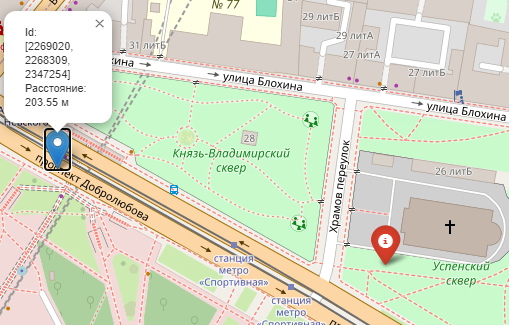
\includegraphics[width=0.6\textwidth]{haversine.png}
        \caption{Результаты вычисления расстояний с помощью формулы гаверсина}
        \label{fig:haversine_vs_yandex}
    \end{figure}
    \begin{figure}[H]
        \centering
        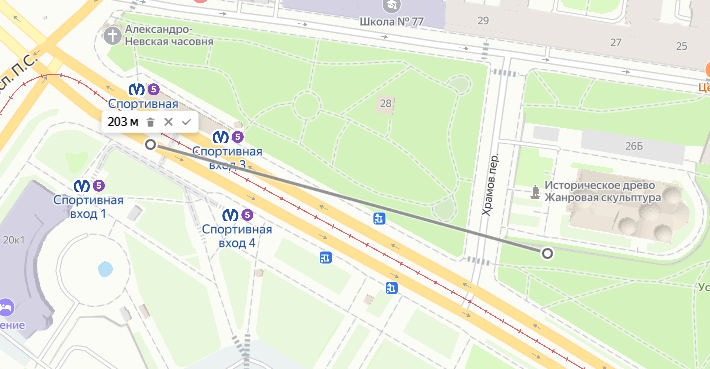
\includegraphics[width=0.8\textwidth]{yandex.png}
        \caption{Результаты вычисления расстояний на Яндекс.Картах}
        \label{fig:yandex_vs_haversine}
    \end{figure}

    \subsection*{3.2. Преобразование координат в декартову систему}

    Поскольку формулы триангуляции предполагают работу в плоской системе координат,
    координаты всех вышек преобразуются в систему \((x, y)\) в метрах с помощью простой цилиндрической проекции:
    Так как вышки рядом, это позволяет достичь необходимой точности и избежать искажений.

    \begin{itemize}
        \item Центром проекции выбирается средняя широта и долгота ближайших станций;
        \item Широта проецируется линейно, долгота — с учётом \(\cos(\phi_0)\) для корректировки искажения.
    \end{itemize}

    \subsection*{3.3. Алгоритмы определения позиции}

    Алгоритм выбора зависит от количества ближайших станций:

    \begin{itemize}
        \item \textbf{Если две станции}: используется метод пересечения окружностей (триангуляция по двум точкам),
        который возвращает две возможные точки. При расчёте метрик выбирается ближайшая к фактической.
        \item \textbf{Если три и более станций}: применяется метод наименьших квадратов.
        Он строит переопределённую систему линейных уравнений, приближая точку по всем окружностям сразу.
    \end{itemize}

    \subsubsection*{Триангуляция}

    Данный подход хорошо работает даже при наличии небольших ошибок в данных
    — благодаря устойчивости метода наименьших квадратов. На Рисунке 3 показан пример работы
    алгоритма на трёх станциях.
    \begin{figure}[H]
        \centering
        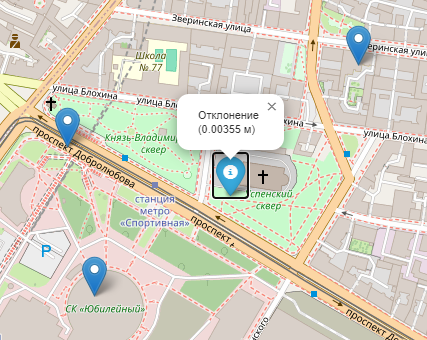
\includegraphics[width=0.7\textwidth]{triangulation.png}
        \caption{Пример работы алгоритма на трёх станциях}
        \label{fig:triangulation_example}
    \end{figure}

    \subsubsection*{"Дуогуляция"}

    Если доступны только две станции, определяется точка пересечения двух окружностей.
    Алгоритм геометрически строит возможные точки, лежащие на пересечении.
    Результат изображён на Рисунке 4.
    \begin{figure}[H]
        \centering
        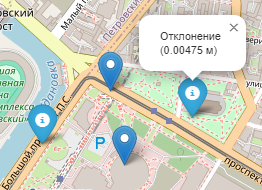
\includegraphics[width=0.7\textwidth]{dougulation.png}
        \caption{Пример работы алгоритма дуогуляции}
        \label{fig:duogulation_example}
    \end{figure}



    \subsection*{3.4. Оценка точности и вычисление ошибок}

    После предсказания координат пользователя, расстояние до истинной позиции оценивается функцией гаверсина.
    Далее вычисляются метрики:

    \begin{itemize}
        \item Средняя ошибка;
        \item Медианная ошибка;
        \item Нормированная ошибка (на 50 м);
        \item Процент попаданий в радиус 50 м.
    \end{itemize}

    Итоговая таблица (Рисунок 5) ошибок позволяет оценить,
    насколько хорошо работает алгоритм в реальных условиях.
    \begin{figure}[H]
        \centering
        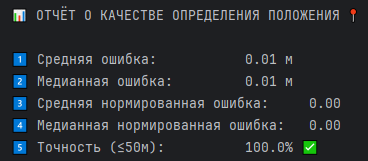
\includegraphics[width=0.8\textwidth]{errors.png}
        \caption{Таблица ошибок предсказания для поиска вышек на расстоянии до 500 метров}
        \label{fig:errors_table}
    \end{figure}

% =============================================
% Вывод
% =============================================
    \section*{4. Заключение}
    Разработанный алгоритм успешно решает задачу определения положения абонента на плоскости
    по координатам и расстояниям до ближайших вышек сотовой связи.
    Использование метода гаверсина обеспечивает высокую точность расчётов расстояний,
    а цилиндрическая проекция позволяет корректно преобразовывать координаты в декартову систему.
    Алгоритмы триангуляции и мультилатерации позволяют эффективно определять положение абонента
    в зависимости от доступных данных о вышках. В итоге полученные результаты показывают, что отклонение
    от истинной позиции в среднем составляет менеe 10 сантиметров,
    что является отличным результатом для данной задачи.

\end{document}

